\documentclass[11pt]{article}

\usepackage[letterpaper, margin=1in]{geometry}

\usepackage[spanish]{babel}
\usepackage[utf8]{inputenc}
\usepackage{multirow}
\usepackage{tabularx}
\usepackage{longtable}



%Figuras
\usepackage{graphicx, subfigure}
\usepackage[]{tikz}
\usepackage{pbox}

%Matemática
\usepackage{amsmath}
\usepackage{amssymb}

%Símbolos mate extra (alfabetos, etc.)
\usepackage{mathrsfs}


%Algoritmos
\usepackage{float}
\usepackage{algorithm}
\usepackage{algorithmicx}
\usepackage{algpseudocode}
\usepackage{listings}


\usepackage{color}
\usepackage{hyperref}

\usepackage{mdframed}
\usepackage{tcolorbox}
\usepackage{multicol}
\usepackage{booktabs}
\usepackage{tabulary}
\definecolor{darkblue}{rgb}{0 , 0.054 , 0.196}



\title{Sobrecarga Operadores- Polinomio}
\author{Leonardo Hern\'andez Chac\'on   - B43262}

\begin{document}

\maketitle
\hrule
\hrule
\tableofcontents
\hspace{5mm}
\hrule
\hrule


\section{Enunciado}

Implemente una clase en C++ que modele polinomios, utilizando sobrecarga de operadores que efect\'ue las cuatro operaciones b\'asicas algebraicas:
   \begin{itemize}
   \item P\& operator+(const P \&rhs); //Suma
   \item P\& operator-(const P \&rhs); //Resta
   \item P\& operator*(const P \&rhs); //Multiplicaci\'on
   \item P\& operator/(const P \&rhs); divisi\'on 
  
   \end{itemize}

Para la divisi\'on, utilice el m\'etodo de la divisi\'on sint\'etica con sus restricciones.

Adem\'as programe los m\'etodos necesarios para que estos operaciones funcionen: Impresi\'on, construcci\'on de copia, asignaciones, etc. 

Haga un programa de prueba en donde se creen objetos e interact\'uen entre ellos.

\section{Desglose}


 \begin{itemize}
   \item main.cpp 
   \item Polinomio.cpp
   \item Polinomio.hpp
   \end{itemize}





\section{main.cpp}
\begin{lstlisting}[language=C]
#include <iostream>
#include "Polinomio.hpp"
using namespace std;


int main(int argc, char** argv)
{
//Creamos Primer Objeto Polinomio
double data0[2]= {2.0,1.0};
int Size0=2;

Polinomio* p0 = new Polinomio(data0, Size0);

//Creamos Segundo Objeto Polinomio
double data1[4]= {8.0,-4.0,2.0, 1.0};
int Size1=4;

Polinomio* p1 = new Polinomio(data1, Size1);

//A continuación, se inician las pruebas 
//Mostrar que los operadores sobrecargados
//Funcionan correctamente

cout <<"Primer Polinomio"<< endl; 
p0->Imprimir();

cout <<"Segundo Polinomio"<< endl; 
p1->Imprimir();

cout <<"//////////////////////////////////"<< endl; 
 

//SUMA:
Polinomio* c = new Polinomio(data1, Size1);
cout <<"Suma"<< endl;
*c =  *p1 + *p0 ;
c->Imprimir();

//RESTA
cout <<"Resta"<< endl;
*c =  *p1 - *p0 ;
c->Imprimir();

//MULTIPLICACION
cout <<"Multiplicacion"<< endl;
*c =  *p1 * *p0 ;
c->Imprimir();

//DIVISION
cout <<"Division"<< endl;
*c =  *p1 / *p0 ;
c->Imprimir();

delete p0;
delete p1;
delete c;


return 0;

};

\end{lstlisting}


\section{Polinomio.cpp}
\begin{lstlisting}[language=C]
#include "Polinomio.hpp"

//Destructor
Polinomio::~Polinomio(){


}

//Constructor
//Recibe un int tamaño, que equivale al grado -1.
//Recibe un arreglo, que le pasa los coeficientes
Polinomio::Polinomio(double arr[], int Size){

    
    this->Size= Size;
    data= new double[Size];
    for(int i=0; i<Size; i++){
    	data[i]= arr[i];
	}
}


//Permite imprimir un polinomio.

void Polinomio::Imprimir(){

	for(int i=0; i<Size; i++){
			cout << data[i] << " ";
		}
			cout << endl;

}



//Se sobrecarga el operador = que más adelante es necesario
//Para hacer las pruebas
Polinomio& Polinomio::operator=(const Polinomio &rhs) {
     this->Size = rhs.Size;

	for(int i=0; i<rhs.Size; i++){
		    data[i]= rhs.data[i];
		}

    return *this;
}


//Se sobrecarga el operador +
Polinomio& Polinomio::operator+(const Polinomio &rhs) {
	//Se determina el tamaño del polinomio resultante
	//tomando en cuenta cual es más grande y asignando 
	//ese.
       int SizeRes=0;
       if (Size > rhs.Size){
		SizeRes= Size;
	}
	else{
		SizeRes= rhs.Size;
	}

	double dataRes[SizeRes];
	for (int c = 0; c < SizeRes; c++) {
            dataRes[c] = data[c] + rhs.data[c];
        }
	
	//Retornamos un polinomio, a la operación suma
    	Polinomio* p = new Polinomio(dataRes, SizeRes);  
    return *p;
}

//Sobrecargamos el operador resta. Muy similar a la suma. 
Polinomio& Polinomio::operator-(const Polinomio &rhs){
	int SizeRes=0;
       if (Size > rhs.Size){
		SizeRes= Size;
	}
	else{
		SizeRes= rhs.Size;
	}

	double dataRes[SizeRes];


	 if (Size >= rhs.Size){
			for (int c = 0; c < rhs.Size; c++) {
           		 dataRes[c] = data[c] - rhs.data[c];
        		}
			for (int c = rhs.Size; c < SizeRes; c++) {
           		 dataRes[c] = data[c];
        		}
	 }
	 else{
		        for (int c = 0; c < Size; c++) {
           		dataRes[c] = data[c] - rhs.data[c];
        		}
			for (int c = Size; c < SizeRes; c++) {
           		 dataRes[c] = -1 * rhs.data[c];
        		}
	 }
	//Retornamos un polinomio, a la operación resta
    	Polinomio* p = new Polinomio(dataRes, SizeRes);  
        return *p;
}

//Sobrecargamos el operador multiplicacion.
Polinomio& Polinomio::operator*(const Polinomio &rhs){
    int SizeRes=(Size + rhs.Size -1);

    double dataRes [Size + rhs.Size - 1]; 
	//LLenamos el arreglo dataRes con 0. Como valor inicial.
    for (int c = 0; c < Size + rhs.Size - 1; c++)
        dataRes[c] = 0;
	//Sumamos a dataRes los términos multiplicados que equivalen al grado
	//de la equiz asociada a esa posición. 
   for (int a = 0; a < Size; a++){
        for (int b = 0; b < rhs.Size; b++){
           dataRes[a+b] += data[a] * rhs.data[b];  
        }
    }

	//Retornamos un polinomio, a la operación multiplicacion
    	Polinomio* p = new Polinomio(dataRes, SizeRes);  
        return *p;
}

//Para sobrecargar el metodo division, utilizamos división sintética
//Cabe destacar que si el divisor no es un monomio, no es válido 
//Utilizar esta técnica.

//Además para esta técnica se omite el residuo.

Polinomio& Polinomio::operator/(const Polinomio &rhs){
int SizeRes= Size -1;

double dataRes [SizeRes]; 
//Se llena dataRes con 0.
for (int c = 0; c < SizeRes; c++)
	dataRes[c] = 0;
//Se verifica que el divisor ser un monomio
if (rhs.Size!= 2){
cout << "No es posible aplicar division sintetica" << endl;
}


else{
double coef= -1* rhs.data[0];


for (int c = 0; c < SizeRes; c++)
	if(c==0){
	//cout<< "data[SizeRes-c+1]"<<data[SizeRes-c+1]<< endl;
	dataRes[SizeRes-c-1] = data[SizeRes-c];
	
	}
	else{
dataRes[SizeRes-c-1] = data[SizeRes-c]+ (dataRes[SizeRes-c]*coef);
	}


}
//Retornamos un polinomio, a la operación division
Polinomio* p = new Polinomio(dataRes, SizeRes);  
return *p;

}



\end{lstlisting}

\section{Polinomio.hpp}
\begin{lstlisting}[language=C]
#ifndef POLINOMIO_HPP
#define POLINOMIO_HPP

#include <iostream>

using namespace std;

class Polinomio {
	public:
		
		//metodos
		Polinomio(double data[], int Size);
		virtual ~Polinomio();
		void Imprimir();

		//Atributos:
		int Size; 
		double* data;

	//Sobrecarga Operadores:
	Polinomio& operator=(const Polinomio &rhs);
        Polinomio& operator+(const Polinomio &rhs);
	Polinomio& operator-(const Polinomio &rhs);
	Polinomio& operator*(const Polinomio &rhs);
	Polinomio& operator/(const Polinomio &rhs);
     
	
};



#endif /* POLINOMIO_HPP */


\end{lstlisting}

\section{Conclusiones}
Para mostrar el funcionamiento, se crearon dos polinomios de tamaño diferente, y los cuales interactuaron realizando las cuatro operaciones elementales, con los operadores sobrecargados. Cabe señalar que se manejo los polinomios en vectores en donde su posici\'on en dicho vector indica la potencia de la variable, es decir el valor en lo posici\'on 0 es la constante, en la posici\'on 1 es X, y así sucesivamente.
A continuaci\'on se muestra los resultados, que puden ser vistos en pantalla luego de correr el makefile incluido. 

\begin{figure}[ht]
\centering
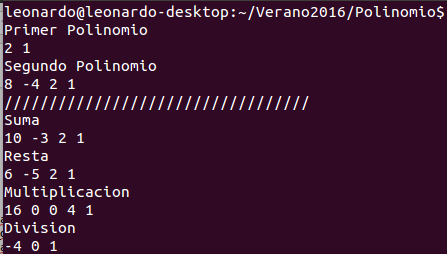
\includegraphics[scale=0.4]{ressss.png}
\caption{Resultados}
\end{figure}


\end{document}